\chapter{Scale, Flow, and the Arithmetic of Durable Wealth}

This chapter comes from a School of Hard Knocks conversation with Grant Cardone, curated into companion-note form by LazyingArt LLC with Video2Book. It is not a classroom lecture in economics. It is, however, organized by a real arithmetic: how large the money pool is, how thin a million dollars becomes when spread across time, how fragile small systems are, and how scale alters both business and life. The interview unfolds in that order. It opens with a cold denominator, moves through boredom and urgency, then turns to lifetime-spending arithmetic, durable wealth, audience, real-estate scale, and finally to conversion, reinvestment, and routine.

\section{A Tiny Slice of a Huge Money Pool}

The lecture begins before the host introduction, and that beginning sets the scale of everything that follows. Cardone does not first define success psychologically. He first describes a channel: he builds a large audience, creates offers, and then invites that audience to invest. The first mathematical object is therefore not a wage or a savings goal, but a denominator.

He says that he has raised \$1.1 billion through crowdfunding on the internet and that he thinks against a pool of roughly \$80 trillion of U.S. dollars in circulation. The point is not a monetary theorem. The point is comparative scale.

\begin{equation}
T_{\$}=80\times 10^{12},
\qquad
s(W)=\frac{W}{T_{\$}}.
\end{equation}

Here \(T_{\$}\) is the dollar pool he invokes, and \(s(W)\) is the share of that pool represented by a target wealth \(W\). If we write out the arithmetic that his opening speech implies, we get

\begin{align}
s(10^6) &= \frac{10^6}{80\times 10^{12}} = 1.25\times 10^{-8},\\
s(10^9) &= \frac{10^9}{80\times 10^{12}} = 1.25\times 10^{-5}.
\end{align}

The lecture's claim is then easy to state. A million dollars and even a billion dollars are not the whole of the universe. They are tiny claims on an enormous stock. Once we take that point seriously, the phrase ``I need a tiny piece'' ceases to be theatrical and becomes operational.

Already in this cold open a second corollary appears. Cardone says that if one has zero money, one does not yet have a \emph{money problem} in the interesting sense; one has absence. The game begins when there is enough flow, enough capital, and enough exposure for management, deployment, and loss to matter. This too will return.

\section{Boredom, Urgency, and the Destruction Loop}

Only after the teaser does the interview reset into its first explicit question. The host asks about free time, cheap entertainment, addiction, and self-improvement. Cardone answers with a causal structure rather than a therapeutic one. Boredom is not merely an idle mood. In his telling, it is the condition under which compromise enters.

\begin{equation}
\text{boredom} \to \text{compromise} \to \text{trouble},
\qquad
\text{urgency} \to \text{schedule} \to \text{production}.
\end{equation}

This compressed diagram is rough, but it does real work. The lecture is heading toward large numbers, but it refuses to separate those numbers from the habits that would be required to survive them. Free time becomes dangerous because it invites leakage: drugs, drift, bad company, wasted nights, and eventually lost productive capacity. Urgency becomes valuable because it organizes the day before compromise has a chance to enter.

The result is that the moral tone of the interview is not a detachable outer layer. It is part of the arithmetic. A billion dollars, in Cardone's language, is not a single lucky jump from one number to another. It is the result of repeated competent action, repeated restraint, and repeated redeployment. That is why the first answer spends so much time on sleep, waking early, moving, meeting, and surrounding oneself with people who are already in motion. Before the lecture asks how much money freedom requires, it asks what kind of life could carry repeated effort long enough to matter.

\section{A Million Dollars Is Still No Money}

The interview now arrives at its first sharp numerical obstacle. The host recalls Cardone's claim that if one plans to live on a million dollars, one is not wealthy but worried. Here the rhetoric tightens into a worked example.

\subsection{Question \& Answer}

\paragraph{Question.}
Why is a million dollars not yet freedom?

\paragraph{Answer.}
Cardone answers by converting a stock into a monthly flow. He asks the listener's age, asks how long the listener expects to live, and then divides the million by the remaining months.

If we follow the values spoken in the interview, we take current age \(21\), terminal age \(80\), and therefore

\begin{align}
N_m &= (80-21)\times 12 = 708,\\
\frac{1{,}000{,}000}{N_m}
&= \frac{1{,}000{,}000}{708}
\approx 1{,}412\ \text{USD/month}.
\end{align}

The calculation is intentionally harsh. There is, in the setup, no inflation, no medical shock, no political shock, no accident, and no ordinary stupidity. Even under those charitable assumptions the monthly draw is narrow. The lecture's point is immediate: one million dollars is too thin to support the emotional prestige that popular culture attaches to it.

At this point the cold-open remark about ``money problems'' becomes clearer. Zero dollars is not yet a complicated capital-allocation problem. The complicated problem begins once there is money enough to be insufficient in subtle ways.

The lecture then scales the same demystification upward. Cardone asks how many times one must make and retain a million dollars in order to keep a billion. A clean way to write the estimate is to let \(r\) denote the retained fraction of each gross \$1 million after taxes, payroll, and leakage. Then

\begin{equation}
N_{\text{gross million wins}}
=
\frac{10^9}{r\cdot 10^6}
=
\frac{1000}{r}.
\end{equation}

If \(r\) is modest, the required number of gross million-dollar events is indeed in the thousands. This is the precise mathematical version of his remark that one must do it ``thousands and thousands of times, and not blow it.'' The point is not the exact number. The point is that the jump from millionaire fantasy to durable billion-dollar scale is not a single step.

One further motivational beat should be preserved here. Cardone says, in effect, that if one is broke, one should stop having firm opinions about money. The chapter should hear that line not as humiliation for its own sake, but as a demand to let arithmetic break inherited reference points.

\section{From Poor to Rich to Wealthy}

Once the prestige of the million has been punctured, the lecture broadens into a state model. The old comparison to parents, grandparents, and neighbors is rejected. Instead the opening denominator returns: compare yourself to the size of the money pool, then ask what kind of structure you are actually building.

\begin{definition}
In the working vocabulary of this interview, \emph{rich} means high present income tied to a person, job, or active operator, while \emph{wealthy} means a durable structure of assets, enterprise, or brand that can continue when that operator disappears.
\end{definition}

The lecture's path through states is then

\begin{equation}
\text{poor}\to\text{middle class}\to\text{rich}\to\text{wealthy}.
\end{equation}

The middle class appears here not as an endpoint but as a temptation: air conditioning, cars, some entertainment, a visible improvement over earlier poverty, and therefore the dangerous belief that the problem has been solved. Rich comes next: the large salary, the club, the larger house, the visible markers, the tax burden, and still, perhaps, no real freedom.

The proof is autobiographical and should remain where it appears in the transcript. Cardone says that his father died young, the income stopped, and within a matter of days the family situation changed. This is not a decorative memory. It is the lecture's local proof that high inflow is not yet durable structure.

\begin{figure}[h]
\centering
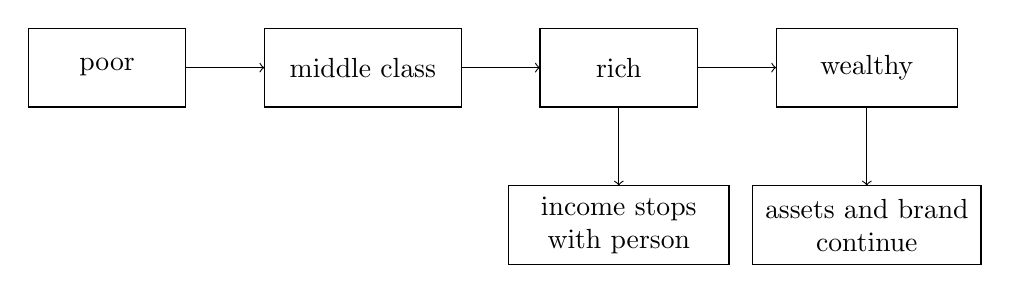
\begin{tikzpicture}[x=1cm,y=1cm]
\draw (0,0) rectangle (2,1);
\node at (1,0.5) {poor};

\draw (3,0) rectangle (5.5,1);
\node at (4.25,0.5) {middle class};

\draw (6.5,0) rectangle (8.5,1);
\node at (7.5,0.5) {rich};

\draw (9.5,0) rectangle (11.8,1);
\node at (10.65,0.5) {wealthy};

\draw[->] (2,0.5) -- (3,0.5);
\draw[->] (5.5,0.5) -- (6.5,0.5);
\draw[->] (8.5,0.5) -- (9.5,0.5);

\draw (6.1,-2) rectangle (8.9,-1);
\node[align=center] at (7.5,-1.5) {income stops\\with person};
\draw[->] (7.5,0) -- (7.5,-1);

\draw (9.2,-2) rectangle (12.1,-1);
\node[align=center] at (10.65,-1.5) {assets and brand\\continue};
\draw[->] (10.65,0) -- (10.65,-1);
\end{tikzpicture}
\end{figure}

This figure simply makes explicit the logic already embedded in the interview. Rich can still be mortal in the narrowest financial sense. Wealth is the attempt to construct continuation.

It is here that Cardone's later emphasis on brand should be understood. Brand is not merely attention. It is one of the devices by which the economic structure is made to outlive the original body.

\section{The Way to Money Is Through People}

After classifying states of wealth, the lecture turns to mechanism. The mechanism is almost embarrassingly simple: money comes through people.

\begin{definition}
The conduit principle of the lecture is this: money does not arrive in a human life except through another human being.
\end{definition}

The credit-card demonstration makes the point in miniature. One can either steal once, or one can create a relationship that opens repeated access. The lecture is clear about which of these counts as an actual business mechanism. The channel is the substance.

We should therefore hear the next turn of the interview as a continuation rather than a change of subject. Cardone is asked about the best financial advice he ever received, and he answers with the lesson he says he learned in \emph{Undercover Billionaire}. The problem was framed as follows: take \$100 and build a business. He rejects the frame. If the target is \$10 million, then the problem is not how to preserve the \$100 but how to stop thinking like the custodian of a trivial sum.

That is why he says the fastest way from \$100 to \$10 million is, in effect, to go to zero immediately. It is a dramatic way of saying that careful management of the tiny stock obstructs clear vision of the real mechanism. He says he needs people, not money; the relevant operation is to raise capital and deploy it, not to sit guarding a small pile.

\begin{equation}
\text{audience} \to \text{offer} \to \text{customer/investor} \to \text{capital}.
\end{equation}

\begin{figure}[h]
\centering
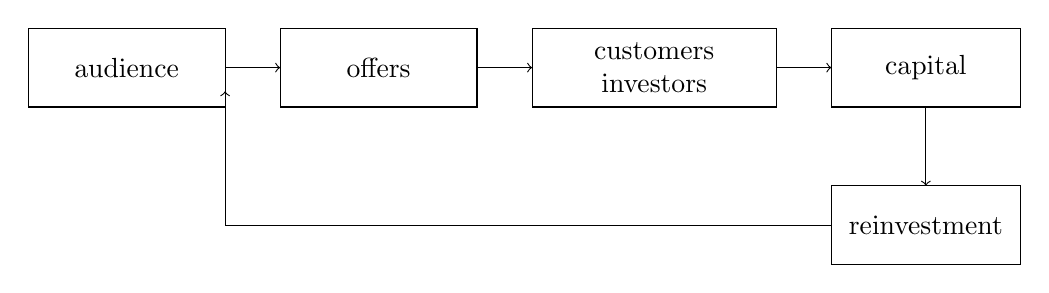
\begin{tikzpicture}[x=1cm,y=1cm]
\draw (0,0) rectangle (2.5,1);
\node[align=center] at (1.25,0.5) {audience};

\draw (3.2,0) rectangle (5.7,1);
\node[align=center] at (4.45,0.5) {offers};

\draw (6.4,0) rectangle (9.5,1);
\node[align=center] at (7.95,0.5) {customers\\investors};

\draw (10.2,0) rectangle (12.6,1);
\node[align=center] at (11.4,0.5) {capital};

\draw (10.2,-2) rectangle (12.6,-1);
\node[align=center] at (11.4,-1.5) {reinvestment};

\draw[->] (2.5,0.5) -- (3.2,0.5);
\draw[->] (5.7,0.5) -- (6.4,0.5);
\draw[->] (9.5,0.5) -- (10.2,0.5);
\draw[->] (11.4,0) -- (11.4,-1);
\draw[->] (10.2,-1.5) -- (2.5,-1.5) -- (2.5,0.2);
\end{tikzpicture}
\end{figure}

It helps to picture the lecture's operating logic in this way. The audience is not an ornament attached to the business. It is one of the business's central capital-forming devices.

This is also why the brand section arrives where it does. Cardone's advice about brand is not advice about polish. It is advice about repeated visibility. One is building a brand anyway. The task is to keep showing up until a public channel exists. His line ``as long as you call me'' compresses a great deal: recognition is already economic access.

The high-school story about the man who fought every Friday and never won serves a parallel function. The man became dangerous not by mastery but by repeated presence. Cardone extracts the business version of the lesson: one keeps showing up until repeated presence itself changes the field.

\section{One House Does Not Scale}

The interview now arrives at its first long worked business example. The host proposes a jump from a one-unit deal to a much larger second deal. Cardone interrupts and corrects the sequence: the first deal was single-family, the second deal was also single-family, and the third deal, after a delay of years, was the 48-unit property. The correction matters because the whole lesson depends on the sequence of discovery.

\subsection{Question \& Answer}

\paragraph{Question.}
Why does a single house fail as a scalable wealth machine?

\paragraph{Answer.}
Because its cash flow is too local and too fragile. One tenant can make the income appear; one vacancy can erase it.

This is exactly how the lecture explains the problem. The speaker imagines a named tenant, imagines her paying rent, and then imagines her moving out. When she leaves, the money disappears. That is the bottleneck. Hence the sentence that solves the local problem: do not buy one unit.

The first single-family deal still matters. Its roughly \$200 per month of cash flow teaches that money can be produced outside the narrow world of a commission check. But the lecture insists that this is only a first opening, not the final mechanism, because the system does not scale. At this point Cardone explicitly contrasts small local success with scalable structures and says, in substance, that Amazon scales.

The narrative rhythm then matters. The first two deals are close together; the large deal comes three years later. Study fills the gap. He spends time learning the asset class, then recognizes the 48-unit opportunity, raises money, signs the note, and closes.

The secure quantities stated in the interview are these:

\begin{align}
E &= 350{,}000,\\
D &= 1.9\times 10^6,\\
P &\approx 3.7\times 10^6.
\end{align}

From these numbers we may derive, cautiously, a ratio that helps explain the force of the story:

\begin{equation}
\frac{P}{E}\approx \frac{3.7\times 10^6}{350{,}000}\approx 10.6.
\end{equation}

This is not a number spoken directly in the interview. It is simply the explicit ratio hiding inside the values that are spoken. The ratio makes plain why the lecture treats this deal as a change of life rather than as a modest extension of the earlier houses.

Cardone himself then performs the next move in the imagination. If a single deal can produce about \$3.7 million, then ten such events produce

\begin{equation}
10\cdot P \approx 10\cdot 3.7\times 10^6 = 3.7\times 10^7.
\end{equation}

The arithmetic is simple, but again it matters because it shows the change in horizon. One does not yet think about 12,000 units or a multibusiness empire. One first sees that repeating a scalable structure several times leads to a different world.

\begin{remark}
One line in this section of the transcript about the 48-unit property ``earning \$48,000 a month'' and then ``making \$1,000'' is garbled. It is better to stay with the quantities that are clear. The financing lesson, however, is secure: the bank lends against the apartment LLC and the asset structure, not merely against a personal retail credit score.
\end{remark}

\begin{figure}[h]
\centering
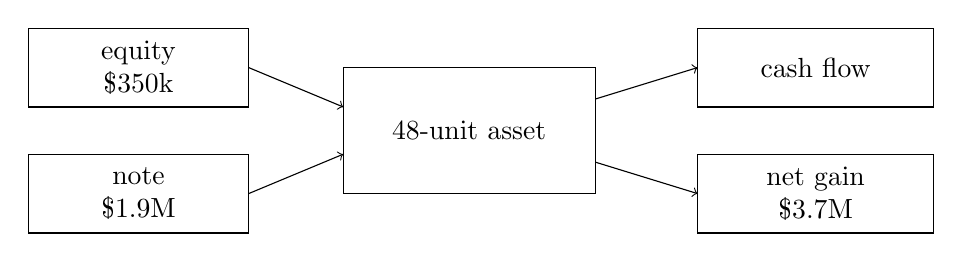
\begin{tikzpicture}[x=1cm,y=1cm]
\draw (0,0.8) rectangle (2.8,1.8);
\node[align=center] at (1.4,1.3) {equity\\\$350k};

\draw (0,-0.8) rectangle (2.8,0.2);
\node[align=center] at (1.4,-0.3) {note\\\$1.9M};

\draw (4,-0.3) rectangle (7.2,1.3);
\node[align=center] at (5.6,0.5) {48-unit asset};

\draw (8.5,0.8) rectangle (11.5,1.8);
\node[align=center] at (10,1.3) {cash flow};

\draw (8.5,-0.8) rectangle (11.5,0.2);
\node[align=center] at (10,-0.3) {net gain\\\$3.7M};

\draw[->] (2.8,1.3) -- (4,0.8);
\draw[->] (2.8,-0.3) -- (4,0.2);
\draw[->] (7.2,0.9) -- (8.5,1.3);
\draw[->] (7.2,0.1) -- (8.5,-0.3);
\end{tikzpicture}
\end{figure}

\section{Scale, Conversion, and the Endgame}

The final long movement of the lecture begins before the ad break and ends with a routine. That is the correct way to hear it. The counts and the life belong together.

\paragraph{Before the break.}
Having shown what a scalable asset looks like, the lecture widens once more. Commitment is placed above excuses. Asset logic is placed above credit-score logic. The educational system is criticized for teaching too much detached material and not enough direct orientation toward building net worth. The speaker then asks what kinds of industries absorb vast demand. Health care, cosmetics, pornography, alcohol, tattoos, and the lottery appear here not because they form a coherent moral family, but because they reveal what large populations visibly buy.

The cleanest number in this portion is the annual lottery figure:

\begin{equation}
L = 105\times 10^9\ \text{USD/year}.
\end{equation}

The lecture's point is not to admire the lottery but to notice the size of the flow. People spend extraordinary amounts of money around the hope of a win. The same logic then produces the comparison between visible abs and millionaires:

\begin{equation}
\frac{22\times 10^6}{3\times 10^6}
=
\frac{22}{3}
\approx 7.33.
\end{equation}

The meaning is again comparative, not biological. If one wants to change what seems plausible, one should compare the counts.

The yacht story belongs to the same argumentative movement. The fishing-boat image comes first: if the boats and birds cluster in one place, that is where the fish are. The Mediterranean yacht story is the same image translated upward. If the largest concentrations of wealth have already chosen a location, the lecture says, one should begin by noticing that choice. ``Follow the money'' is the slogan attached to that whole cluster of examples.

\paragraph{After the break.}
Once the interruption ends, the lecture restates its main law in harsher form: if one does not scale, one does not really have a business. Small firms are controlled by small numbers of customers and employees. Large systems can absorb local failure. This is why the lecture links scale to freedom rather than to vanity.

The next turn is then natural. Success attracts talent. A team, a conference, or a company that is already visibly winning can recruit people who want to win. A small group with only an idea struggles both to attract and to retain serious players. This is how the business argument and the personal-discipline argument begin to close into each other.

At this point the cold open returns in fuller numerical form. Cardone says that 80\% of what he does is free, 20\% is paid, and that the paying layer nonetheless produces on the order of \$150 million in annual revenue.

\begin{equation}
f_{\text{free}}=0.80,
\qquad
f_{\text{paid}}=0.20,
\qquad
R_{\text{paid}}\approx 150\times 10^6\ \text{USD/year}.
\end{equation}

He then gives two sets of counts. One concerns investors: about 450,000 people express interest, and about 13,000 invest. The other concerns customers more generally: about 16 million people are reached online, about 154,000 buy something, and about 45,000 become repeat buyers. The spoken percentages are inconsistent, so we keep the counts and correct the arithmetic.

\begin{align}
c_{\text{invest}} &= \frac{13{,}000}{450{,}000} \approx 2.89\%,\\
c_{\text{buy}} &= \frac{154{,}000}{16{,}000{,}000} \approx 0.96\%,\\
c_{\text{repeat}} &= \frac{45{,}000}{154{,}000} \approx 29.2\%.
\end{align}

\begin{figure}[h]
\centering
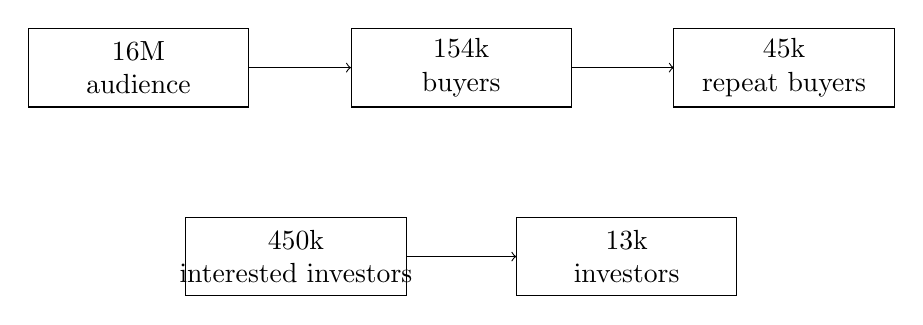
\begin{tikzpicture}[x=1cm,y=1cm]
\draw (0,2.2) rectangle (2.8,3.2);
\node[align=center] at (1.4,2.7) {16M\\audience};

\draw (4.1,2.2) rectangle (6.9,3.2);
\node[align=center] at (5.5,2.7) {154k\\buyers};

\draw (8.2,2.2) rectangle (11,3.2);
\node[align=center] at (9.6,2.7) {45k\\repeat buyers};

\draw[->] (2.8,2.7) -- (4.1,2.7);
\draw[->] (6.9,2.7) -- (8.2,2.7);

\draw (2,-0.2) rectangle (4.8,0.8);
\node[align=center] at (3.4,0.3) {450k\\interested investors};

\draw (6.2,-0.2) rectangle (9,0.8);
\node[align=center] at (7.6,0.3) {13k\\investors};

\draw[->] (4.8,0.3) -- (6.2,0.3);
\end{tikzpicture}
\end{figure}

The lecture's interpretation of these counts is crucial. Closing is not treated as the moment at which the seller traps the buyer. It is the first moment at which the buyer is truly served. That is why the repeat-buyer figure matters. A close opens the real relationship.

The final motivational beat then restores the earlier discipline argument, but now with greater weight. Cardone speaks about the years after his collapse into drugs and bad company, the years of showing up first and leaving last, the refusal to attend late-night parties, and the conscious manufacture of dissatisfaction in order to avoid drift. The rhetoric is severe, but its function is clear. The larger numbers above depend on this smaller order below.

The capital-allocation rule that closes the chapter is therefore simple:

\begin{equation}
\text{earn} \to \text{reinvest in self, business, brand} \to \text{acquire outside real assets}.
\end{equation}

This final rule also clarifies the lecture's insistence that money matters. Hospitals, schools, stores, churches, parents, and children do not accept feeling as payment. They take dollars. The lecture's game of production is therefore not opposed to obligation. It is one proposed way of meeting it.

At the very end the speaker makes a dated market call on Austin real estate, even forecasting purchases far below prior prices. That forecast should remain in the chapter as a claim made in time, not as a timeless proposition. The stable lesson lies deeper: do not stop at self-investment and business-investment. Eventually one must push outward into assets that stand apart from the original operating machine.

\section{Summary}

The interview begins with a denominator and ends with a schedule. In between it constructs a practical arithmetic of wealth. A million dollars becomes a monthly flow and loses its mystique. Rich and wealthy separate once we ask whether income survives the person. Money is said to travel through people, not around them. Small deals can teach, but scalable structures change the order of magnitude. Large demand reveals itself in counts and flows, not in slogans. Free attention becomes paid conversion, and paid conversion must be followed by repeated service.

The mathematics is elementary on purpose. That is why it bites. The lecture's wager is that if we keep the ratios, the transitions, and the conduits in view, wealth begins to look less like magic and more like structure.